\section{Case Study 1: Intelligence Analysis}
\label{sub:ts-vast}
This case study explores how TimeSets supports intelligence analysis, the domain for which it is specifically designed. We integrated TimeSets into the visual analytics system SAVI~\cite{Xu2014} and used it to participate in the IEEE VAST Challenge 2014~\footnote{\url{http://www.vacommunity.org/VAST+Challenge+2014}}. Participants were given a synthetic dataset and asked to identify suspicious activities within that dataset. The particular mini challenge that SAVI involved was about a fictitious company where several employees had been missing. Participants had to collect and analyze streaming tweets in order to identify five \emph{interesting events} before presenting hypotheses and evidence about the disappearance of those employees. With the help of TimeSets, we won an award in Mini Challenge 3. Next, we describe the SAVI interface and how TimeSets contributes to make sense of temporal relationships in the data.

SAVI consists of five linked views (\autoref{fig:ts-savi}). To provide an overview of the dataset, a continuous histogram (\autoref{fig:ts-savi}A) shows the frequency of tweets over time (from 5pm to 9:30pm for this dataset). The histogram can provide initial cues for further investigation such as frequency peaks indicating that interesting events were happening around that time. Selecting the first peak (between 6:30pm to 7pm) makes the corresponding tweets to be displayed in the TimeSets view (\autoref{fig:ts-savi}C), allowing us to quickly read through those tweets and discover that there was a fire at the ``Dancing Dolphin Apartment''.

\begin{figure}[p]
	\centering
	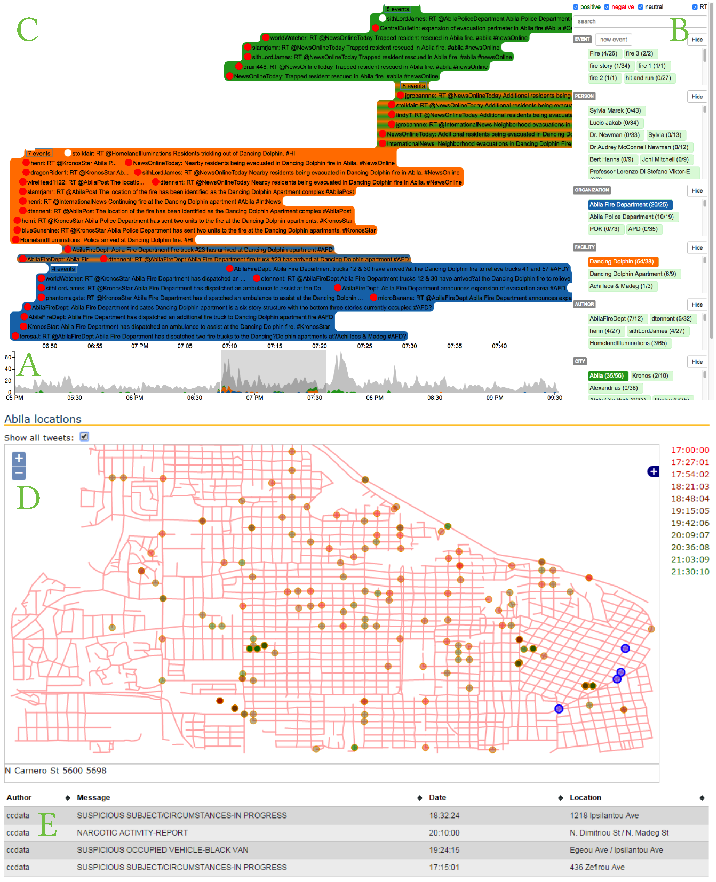
\includegraphics[width=\linewidth]{savi}
	\caption[SAVI interface]{SAVI interface. \textbf{A}: Histogram showing the distribution of tweets. \textbf{B}: Extracted named entities organized by type. \textbf{C}: TimeSets displaying selected tweets. \textbf{D}: Map showing tweets with available geolocation. \textbf{E}: Details of tweets selected in the map.}
	\label{fig:ts-savi}
\end{figure}

\autoref{fig:ts-savi}B displays named entities identified from the tweets and organized by entity type. Initially, entities from the entire dataset are shown, but they are updated according to the selected tweets. This view provides an overview of the main keywords mentioned in those tweets. Both the histogram and the entity collection act as filters. Within the previously selected time range, choosing the three most frequent entities (``Dancing Dolphin'', ``Abila Fire Department'' and ``Abila'') limits the tweets in TimeSets to only those containing at least one of the three keywords. TimeSets uses the entities as \emph{sets}, allowing us to quickly examine the story related to both individual and group of entities over time.

The map view (\autoref{fig:ts-savi}D) shows selected tweets with available geolocation information. Each tweet is displayed as a dot at its location and color-coded by its timestamp. These dots can be selected to reveal their detailed information as shown in \autoref{fig:ts-savi}E. TimeSets and other linked views enable us to explore temporal and spatial events.

Besides supporting data exploration, TimeSets can also help present discovered stories, which are interesting events or narratives in this case (\autoref{fig:ts-interesting-event}). An event is described as a sequence of related tweets organized in a chronological order. During the analysis, we create potential events and add tweets into one or multiple of them. As a result, TimeSets allows us to present an event together with its key elements. Also, visualizing many events simultaneously could reveal tweets that belong to multiple of them, which suggests further exploration to understand their relationship.

\begin{figure}
	\centering
	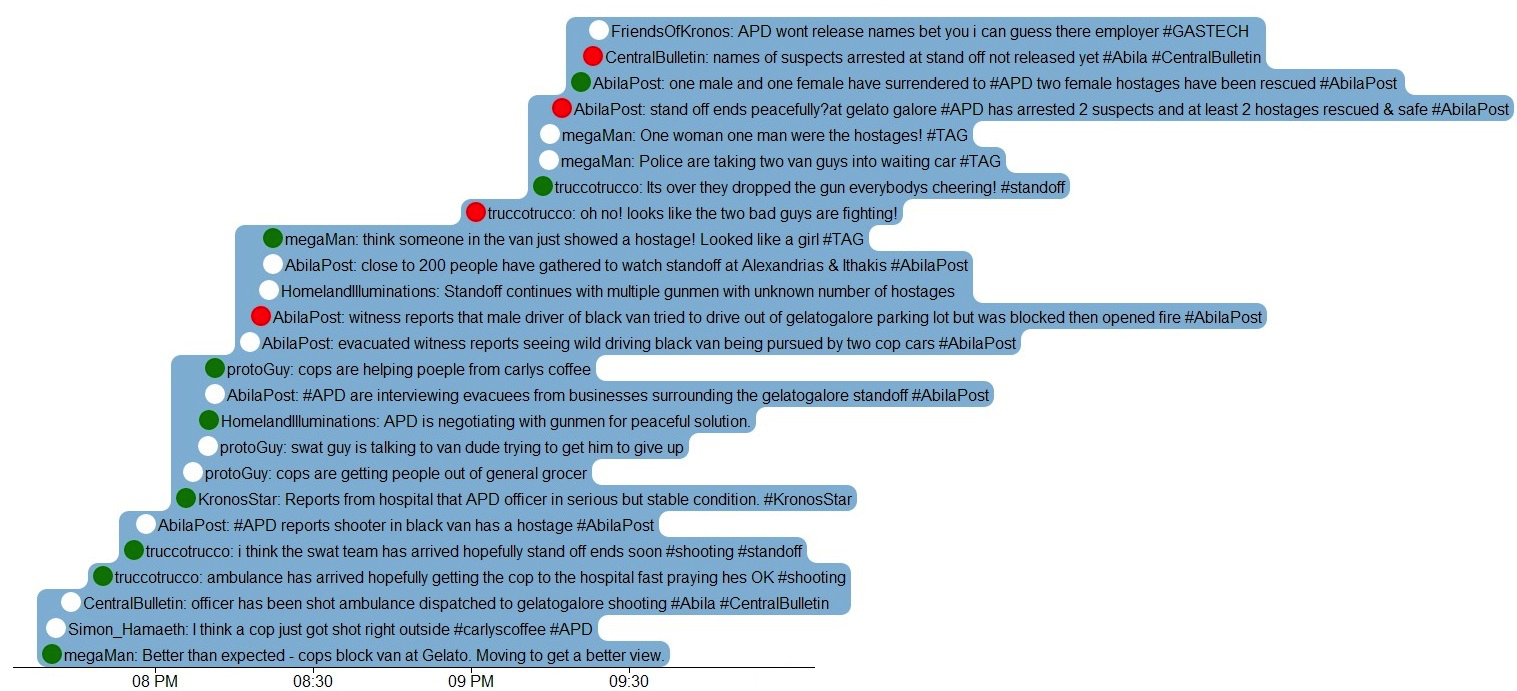
\includegraphics[width=\linewidth]{interesting-event}
	\caption{TimeSets for constructing and presenting an interesting event.}
	\label{fig:ts-interesting-event}
\end{figure}

This case study suggests that TimeSets can be used effectively in supporting intelligence analysis through an application for a VAST Challenge entry. TimeSets was integrated into a visual analytics system (SAVI) for spatial-temporal analysis. It was applied to make sense of tweets in both temporal order and topical categories. It was also used to construct and present interesting stories. In other words, TimeSets showed its flexibility and usefulness of  mapping \emph{set} to different attributes for different purposes.